\subsection{Multi-Head Self-Attention (MSA)}
Introduced in \cite{vaswani2017}. MSA-based networks have shown to be very effective in NLP tasks, such as machine translation, language modeling, and text classification.

\subsubsection{Attention}
The attention function can be understood as a method that takes a query and a collection of key-value pairs and produces an output. All of these elements - the query, keys, values, and output - are vector forms. The output is determined by a weighted sum of the values. Each value's weight is calculated using a compatibility function that matches the query with its associated key.

We can break down the concept of an attention function into:
\begin{itemize}
    \item \textbf{Query, Keys, Values:} These are all vectors. In the context of a transformer model, for example, these vectors are created by multiplying the input vectors (like word embeddings in NLP) with weight matrices that the model learns during training.
    \item \textbf{Mapping:} The attention function maps a query and a set of key-value pairs to an output. This is done through a series of mathematical operations.
    \item \textbf{Compatibility Function:} This is a function that calculates the compatibility or similarity between the query and each key. The result of this function is used to weight the corresponding value. In many models, the dot product is used as the compatibility function.
    \item \textbf{Weighted Sum of Values:} After each value is weighted according to the compatibility of its corresponding key with the query, these weighted values are summed to produce the output. This output is a vector that represents the input elements but with attention applied - elements that are deemed more important (have higher compatibility with the query) have a greater presence in the output.
\end{itemize}

This mechanism allows a model to focus on different parts of the input when producing each part of the output, hence the term "attention". It's a crucial part of many modern neural network architectures, especially in the field of natural language processing.

Attention mechanisms have also been adopted in audio signal processing, particularly in tasks like speech recognition and sound classification. In these tasks, attention mechanisms can help the model focus on certain parts of the audio signal that are more relevant to the task at hand. For instance, in speech recognition, an attention mechanism can allow the model to focus more on the parts of the audio signal where the speech is present and less on the background noise.

\subsubsection{Scaled Dot-Product Attention}
Scaled dot-product attention is a type of attention function that has been used in many NLP models, including the original transformer model. It takes a query and a set of key-value pairs and produces an output. The query, keys, values, and output are all vectors. The output is calculated as a weighted sum of the values, where the weight assigned to each value is calculated using a compatibility function that matches the query with its associated key.

The compatibility function used in scaled dot-product attention is the dot product. The dot product is calculated between the query and each key, then the result is divided by the square root of the dimension of the query vector. This scaling factor is used to prevent the dot product from growing too large, which can cause problems with the softmax function that is used to calculate the weights. The softmax function is a function that takes a vector as input and produces a vector as output, where each element of the output vector is in the range [0, 1] and the sum of the elements is 1. The softmax function is used to calculate the weights assigned to each value in the weighted sum of values that is the output of the attention function.

The scaled dot-product attention function can be expressed as:
\begin{equation} \label{eq:dot-product-attention}
    \text{Attention}(Q, K, V) = \text{softmax}(\frac{QK^T}{\sqrt{d_k}})V
\end{equation}
where $Q$ is the query vector, $K$ is the matrix of key vectors, $V$ is the matrix of value vectors, and $d_k$ is the dimension of the query vector.

\subsubsection{Multi-Head Attention}
Instead of using a single attention function with keys, values, and queries all having a dimension of $d_{model}$, it's found to be advantageous to project the queries, keys, and values h times linearly with different learned linear projections to dimensions $d_k$, $d_k$, and $d_v$ respectively. The attention function is then performed in parallel on each of these projected versions of queries, keys, and values, producing $d_v$-dimensional output values. These outputs are then concatenated and projected again to yield the final values.

This approach, known as multi-head attention, allows the model to attend to information from different representation subspaces at different positions simultaneously. This is something that can't be achieved with a single attention head due to averaging.

Multi-head attention can be expressed as:

\begin{equation} \label{eq:multi-head-attention}
    \text{MultiHead}(Q, K, V) = \text{Concat}(\text{head}_1, ..., \text{head}_h)W^O
\end{equation}

Where $\text{head}_i = \text{Attention}(QW^Q_i, KW^K_i, VW^V_i)$.

Here, the projections are parameter matrices  $W^Q_i \in \mathbb{R}^{d_{model} \times d_k}, W^K_i \in \mathbb{R}^{d_{model} \times d_k}, W^V_i \in \mathbb{R}^{d_{model} \times d_v}, \text{ and } W^O \in \mathbb{R}^{hd_v \times d_{model}}$.

\begin{figure} [ht]
    \centering
    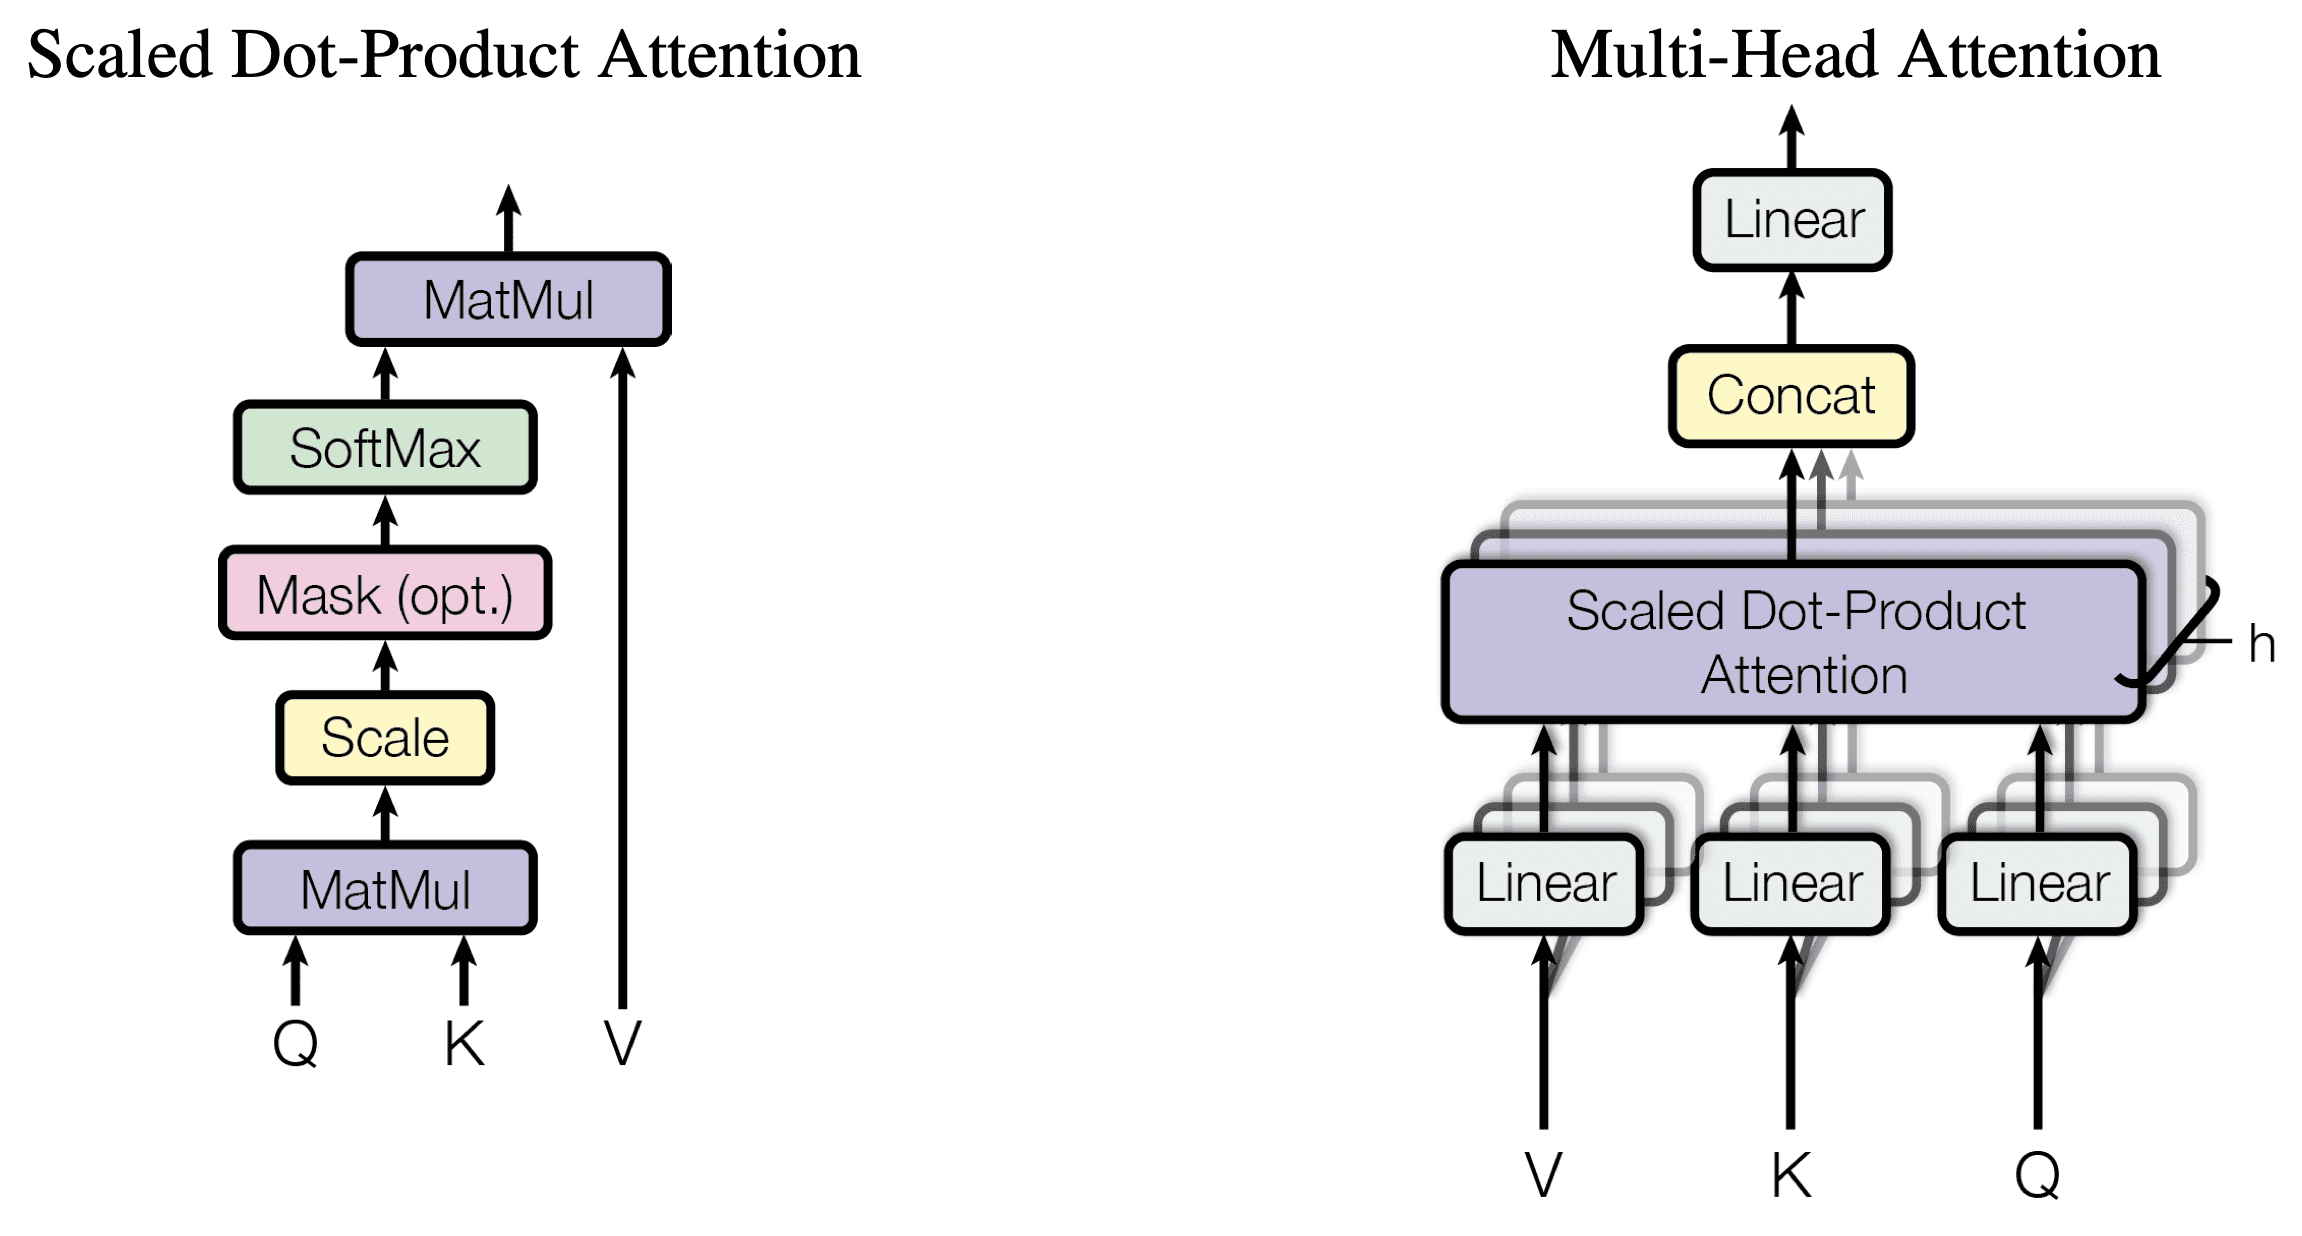
\includegraphics[width=0.75\linewidth]{images/dl/dotproduct.png}
    \caption{(left) Scaled Dot-Product Attention. (right) Multi-Head Attention consists of several
        attention layers running in parallel.}
    \label{fig:attention}
\end{figure}

